\documentclass{beamer}
\usepackage{amsmath,amsthm,amssymb,amsfonts,mathtools}
\usepackage[english]{babel}
%\usepackage[margin=1in]{geometry}
\usepackage{setspace}
%\usepackage{titlesec}
\usepackage{indentfirst}
\usefonttheme{professionalfonts}
\newcommand\Fontvi{\fontsize{8}{7.2}\selectfont}
\usepackage{enumerate}
\usepackage{tikz}
\usepackage{booktabs}
\usepackage{multirow}
\usepackage{tabularx}
%\usepackage{array}
%\usepackage{bm}
%\usepackage{color}
%\usepackage{graphicx}
%\usepackage{xy}

\makeatletter
\g@addto@macro\@floatboxreset\centering
\makeatother

%\titleformat{\section}{\normalfont\bfseries\normalsize}{}{0pt}{}
%\titleformat{\subsection}{\normalfont\bfseries\normalsize}{\thesection (\alph{subsection})}{11pt}{}

\newcommand{\req}[1]{(\ref{#1})}
\newcommand{\be}{\begin{equation}}
\newcommand{\ee}{\end{equation}}
\newcommand{\ba}{\begin{align}}
\newcommand{\EX}{\mathbb{E}}
\newcommand{\Prob}{\mathbb{P}}
\newcommand{\hlinex}{\hline \\ [-2ex]}
\newcommand{\dhlinex}{\hline\hline\ \\ [-2ex]}
\newcommand{\clinex}[1]{\cline{#1} \\ [-2ex]}

\mode<presentation>

\usetheme{Boadilla}

\title[Earnings Forecasts from Firm-Level Regressions: Implications for Research and Practice]{Earnings Forecasts from Firm-Level Regressions: Implications for Research and Practice}
\author[Reginald Edwards]{Reginald Edwards\\2014}
\date[Nov 2014]{Presented: Nov 2014}

\begin{document}

\begin{frame}
\titlepage
\end{frame}

% Overview. Discuss goals of the paper, motivation, related literature, etc.
\begin{frame}
\frametitle{Overview}
Are analyst forecasts of earnings more accurate or more value-relevant than forecasts from statistical models of earnings?
\begin{itemize}
\item How can statistical models incorporate the same information set analysts use?
\item How do we evaluate the performance of a given earnings forecast?
\item When are earnings forecasts likely to perform poorly?
\end{itemize}
\end{frame}

\begin{frame}
\frametitle{Preview of Results}
\begin{enumerate}
\item Analyst forecasts are more accurate at shorter horizons, but statistical forecasts outperform at longer horizons
\item Analyst forecasts underperform statistical forecasts in the period prior to Reg-FD, consistent with a less favorable information environment
\item No clear relation between \emph{ex ante} uncertainty and relative forecast performance
\item Analyst forecasts perform better in high-tech, manufacturing, and healthcare
\item Statistical forecasts associated with marginally better contemporaneous returns
\end{enumerate}
\end{frame}

\begin{frame}
\frametitle{Motivation: Demands for Forecasts of Earnings}
\begin{itemize}
\item Valuation
\item Implied cost of capital
\item Equity risk premium estimates
\item Returns-earnings relations
\item Predictability studies
\end{itemize}
\end{frame}

\begin{frame}
\frametitle{Motivation: Problems with Analyst Forecasts}
\begin{center}
 \begin{figure}
    \includegraphics[height=2.5in, width=3.5in]{../graphics/brown-table8.jpg}
\end{figure}
\end{center}
\emph{Table 8 from Brown, Call, Clement, and Sharp. JAR. (2014)}
\end{frame}

\begin{frame}
\frametitle{Motivation: Problems with Analyst Forecasts}
\begin{itemize}
\item Misaligned incentives of analysts
\item Biased in general (usually over-optimistic)
\item Limited historical availability (late 1980s onward)
\item Limited current availability (large, public firms)
\item Poor performance at long horizons
\end{itemize}
\end{frame}

\begin{frame}
\frametitle{A Brief History of Earnings Forecasting Research}
\begin{itemize}
\item 1960s
\begin{itemize}
\item Random walk models
\end{itemize}

\item 1970s
\begin{itemize}
\item ARIMA time-series models 
\end{itemize}

\item 1980s
\begin{itemize}
\item Incorporating extra information beyond past earnings (eg price)
\item Using analyst forecasts
\item Comparing analysts to time series models
\end{itemize}

\item 1990s
\begin{itemize}
\item Incorporating management forecasts (``guidance'')
\item Assessing biases of analyst forecasts
\end{itemize}
\end{itemize}
\end{frame}

\begin{frame}
\frametitle{A Brief History of Earnings Forecasting Research}
\begin{itemize}
\item 2000s
\begin{itemize}
\item SP Kothari:\\
\begin{quote}``...[earnings forecating] literature is fast becoming extinct. The main reason is the 
easy availability of a better substitute: analysts' forecasts are available at a low cost in
machine-readable form for a large fraction of publicly traded firms''\end{quote}
\end{itemize}

\item 2010s (Today)
\begin{itemize}
\item We can do better.
\end{itemize}
\end{itemize}
\end{frame}

\begin{frame}
\frametitle{Contribution}
\begin{enumerate}
\item Most closely related to Bradshaw et al (2012); Hou, van Dijk, and Zhang (2012); Ball, Ghysels, and Zhou (2014).
\item Methodological innovations in data treatment, model building, and forecast evaluation
	\begin{itemize}
		\item Appropriately map the forecasts to the earnings figures forecast by analysts
		\item Build forecasts at a firm-level rather than from cross-sectional averages
		\item Use a market-based evaluation of forecast performance
	\end{itemize}
\item Demonstrates potential gains to market participants from using statistical forecasts over analyst forecasts
\end{enumerate}
\end{frame}


\begin{frame}
\frametitle{Methodology: Earnings Forecasts}
Which ``earnings'' figure to use?
\begin{itemize}
\item Annual ``pro-forma'' EPS forecasts from IBES
\item Forecasts of one-, two-, and three-year ahead earnings (FY1, FY2, FY3, resp.)
\item Forecasts are made on the base-year announcement date
\end{itemize}
\end{frame}

\begin{frame}
\frametitle{Methodology: Forecasting Framework}
\begin{itemize}
\item Begin with firm-level, first-order autoregressive model and build out:
\begin{equation}
E_{i, t+\tau} = \alpha_{i,0} + \alpha_{i,1} E_{i,t} + \eta_{i,t+\tau},
\end{equation}
where $\tau = 1,2,3$.
\item Add predictor variables to capture firm, market, and economy-wide information
\begin{equation}
E_{i, t+\tau} = \beta_{i,0} + \beta_{i,1} E_{i,t} + \sum_{k=2}^{\kappa} \beta^{(k)}_{i} X^{(k)}_{i, t}  + \varepsilon_{i,t+\tau}
\end{equation}
\end{itemize}
\end{frame}

\begin{frame}
\frametitle{Methodology: Performance Evaluation}
\begin{itemize}
\item Prior studies use bias, absolute error, or mean-square prediction error
\item I use MSPE and buy-and-hold returns
\item Buy-and-hold returns calculated on portfolios ranked by divergence between model and analyst forecasts
\end{itemize}
\end{frame}

\begin{frame}
\frametitle{Methodology: Choosing Predictors}
\begin{itemize}
\item Short earnings histories necessitate parsimony
\item Use prior literature and in-sample correlation to motivate variable selection
\item Be willing to sacrifice in-sample performance for potential out-of-sample performance
\end{itemize}
\end{frame}

\begin{frame}
\frametitle{Methodology: Choosing Predictors}
\begin{itemize}
\item Firm-level data: \begin{itemize}\item Earnings, indicator for negative earnings, assets, sales, ROE, dividends, changes in accruals\end{itemize}
\item \begin{itemize}\item Macroeconomic variables: unemployment, gdp, inflation (ppi)\end{itemize}
\item \begin{itemize}\item Market-based data: price-earnings ratio, year-over-year change in stock price, one year stock price return\end{itemize}
\end{itemize}
\end{frame}

\begin{frame}
\frametitle{Methodology: Choosing Predictors}

\begin{table}
\centering
\Fontvi
\begin{tabular}{rrr}
  \hline
 & mean & med \\
  \hline
$EPS_{t-1}$ & 0.6694 & 0.7516 \\
$\Delta Sales$ & 0.7678 & 0.8687 \\
ROE & 0.7535 & 0.8151 \\
sales & 0.7444 & 0.8100 \\
return & 0.7418 & 0.7834 \\
$\Delta Price$ & 0.7313 & 0.7866 \\
$\Delta AR$ & 0.7195 & 0.7980 \\
$\Delta AP$ & 0.7190 & 0.7868 \\
Inflation (PPI) & 0.7032 & 0.7696 \\
GDP & 0.7046 & 0.7792 \\
Unemployment & 0.7065 & 0.7794 \\
AP & 0.6963 & 0.7648 \\
AR & 0.6925 & 0.7646 \\
Accruals & 0.6923 & 0.7505 \\
Dividends & 0.6953 & 0.7653 \\
assets & 0.6877 & 0.7636 \\
PE Ratio & 0.6843 & 0.7462 \\
Negative Earnings & 0.6797 & 0.7575 \\
   \hline
\end{tabular}
\caption{Estimated $R^2$ values from regressions of the form $EPS_{t} = \alpha_0 + \alpha_{1}EPS_{t-1} + \alpha_{2}X_{t-1} +\varepsilon$.} 
\label{univariate-stats-eps}
\end{table}
\end{frame}

\begin{frame}
\frametitle{Methodology: Forecast Estimation}
\begin{itemize}
\item Regression necessitates relatively long estimation windows. 
\item For firms with at least 15 years of earnings history, use the full feature set:
\begin{equation}
\begin{split}
E_{t+\tau} = \beta_{0} + \beta_{1}E_{t} + \beta_{2}assets_{t} + \beta_{3}return_{t} \\
+ \beta_{4}Negative Earnings_{t} + \beta_{5}PE_{t} \\
+ \beta_{6}\Delta Sales_{t} + \beta_{7}PE_{t} + \beta_{8}\Delta AP_{t} + \\
  \beta_{9}\Delta AR_{t} + \beta_{10}U_{t} \\
+ \beta_{11}GDP_{t} + \beta_{12}INFLATION_{t} + 
  \varepsilon
\end{split}
\end{equation}
\item For short-history firms, fall-back on the AR(1) model.
\item Do not require firms to have positive base-year earnings
%\item Do require earnings not to be negative over the entire estimation window
\end{itemize}
\end{frame}

\begin{frame}
\frametitle{Forecast Evaluation}
Relative MSPE by forecast target year

\begin{table}
\Fontvi
\centering
\begin{tabular}{rcccc}
  \hline
 Year & 1-Year Ahead & 2-Years Ahead & 3-Years Ahead \\ 
\hline
1993 & 0.76 & 0.08 & - \\ 
1994 & 0.9 & 0.11 & - \\ 
1995 & 3.81 & 1.04 & - \\ 
1996 & 24.83 & 0.17 & 0.00 \\ 
1997 & 15.33 & 0.00 & 0.49 \\ 
1998 & 1.17 & 1.23 & 1.81 \\ 
1999 & 8.71 & 0.93 & 1.83 \\ 
2000 & 2.45 & 1.66 & 0.38 \\ 
2001 & 2.01 & 1.25 & 0.09 \\ 
2002 & 0.27 & 0.16 & 0.11 \\ 
2003 & 3.8 & 0.7 & 0.59 \\ 
2004 & 0.83 & 0.46 & 0.64 \\ 
2005 & 0.27 & 0.69 & 0.02 \\ 
2006 & 1.84 & 0.84 & 0.55 \\ 
2007 & 2.37 & 0.97 & 0.77 \\ 
2008 & 1.67 & 1.2 & 0.21 \\ 
2009 & 0.69 & 0.55 & 0.63 \\ 
2010 & 1.29 & 0.57 & 0.45 \\ 
2011 & 1.6 & 0.79 & - \\ 
2012 & 3.13 & 1.12 & - \\ 
2013 & 2.01 &  & - \\ 
\hline
Average & 3.80 & 0.76 & 0.61 \\ 
\hline
\end{tabular}
\caption{Mean squared prediction error of model forecast, mean analyst (MEANEST) forecast. Forecasts are of FY1, FY2, and FY3 earnings.} 
\label{spe-by-year-table-fy1}
\end{table}

\end{frame}

\begin{frame}
\frametitle{Forecast Evaluation}
Two Questions commonly posed of analyst forecasts
\begin{enumerate}
\item Does private information give analysts an advantage? (Gintschel and Markov [2004])
\item Does the amount of \emph{ex ante} uncertainty decrease forecast performance? 
\item Does industry affect forecast performance? 
\end{enumerate}
\end{frame}

\begin{frame}
\frametitle{Results}
\textbf{Relative forecast accuracy after Regulation Fair Disclosure: the effect of private information on forecast performance.}
\begin{table}[H]
\centering
\begin{tabular}{l |  c |  c}
  \hline
Forecast horizon&  \multicolumn{1}{| c}{Pre-Reg FD} &  \multicolumn{1}{| c}{Post-Reg FD} \\
% & Pre-Reg FD & & Post-Reg FD & \\ 
  \hline
%Forecast horizon 	& Pre-RegFD	& Post-RegFD
1-Year Ahead 	& 3.21	& 1.57 \\
2-Year Ahead 	& 0.67	& 1.00 \\
3-Year Ahead 	& 0.43	& 0.46 \\
   \hline
\end{tabular}
\caption{Relative mean squared prediction error comparison of ``model'' and ``consensus'' earnings forecasts.}
\label{evaluation-regfd}
\end{table}
\end{frame}

\begin{frame}
\frametitle{Results}
\textbf{Relative forecast accuracy between high and low analyst forecast dispersion: the effect of \emph{ex ante} uncertainty on forecast performance.}
\begin{table}[H]
\centering
\begin{tabular}{l | c | c }
  \hline
 Forecast horizon&  \multicolumn{1}{| c}{Low Dispersion} &  \multicolumn{1}{| c}{High Dispersion} \\
  \hline
1-Year Ahead 	& 1.92	& 1.84 \\
2-Year Ahead 	& 1.03	& 0.97 \\ 
3-Year Ahead 	& 0.42	& 0.54\\
   \hline
\end{tabular}
\caption{Relative mean squared prediction error comparison of ``model'' and ``consensus'' earnings forecasts.}
\label{evaluation-dispersion}
\end{table}
\end{frame}

\begin{frame}
\frametitle{Results}
\textbf{Industries}
\begin{table}[H]
\Fontvi
\centering
\begin{tabular}{l |  c | c  |  c}
  \hline
&  \multicolumn{1}{| c}{1-Year Ahead} &  \multicolumn{1}{| c}{2-Years Ahead}&  \multicolumn{1}{| c}{3-Years Ahead} \\
  \hline
High-tech  & 1.2 & 1 & 0.9 \\ 
Manufacturing  & 2.2 & 1.1 & 0.4 \\ 
Wholesal/Retail  & 0.9 & 0.9 & 0.4 \\ 
Healthcare  & 1.4 & 1.1 & 0.8 \\ 
Enrgy/Oil/Gas  & 0.9 & 0.7 & 0.2 \\ 
Con Durables  & 4.5 & 1.7 & 0.4 \\ 
Cons Non-Durables  & 0.4 & 1.2 & 0.6 \\ 
other  & 2 & 0.9 & 0.3 \\ 
   \hline
\end{tabular}
\caption{Relative mean squared prediction error comparison of ``model'' and ``consensus'' earnings forecasts by Fama-French Industries.}
\label{evaluation-industry}
\end{table}
\end{frame}

\begin{frame}
\frametitle{Results}
\textbf{Buy and hold returns based on divergence between model and analyst forecasts}
\begin{equation}
BAHR_{t+\tau} = \alpha_{0} + \alpha_{1}DIFF_{i} + \varepsilon.
\end{equation}
\begin{center}
 \begin{figure}
    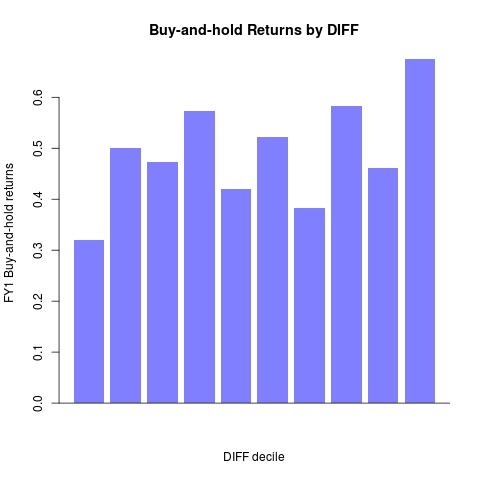
\includegraphics[height=2in, width=3in]{bahr-diff-decile.jpeg}
\end{figure}
\end{center}
\end{frame}

\begin{frame}
\frametitle{Results}
\textbf{Buy and hold returns based on divergence between model and analyst forecasts}
\begin{equation*}
BAHR_{t+\tau} = \alpha_{0} + \alpha_{1}DIFF_{i} + \varepsilon.
\end{equation*}
\begin{center}
 \begin{figure}
    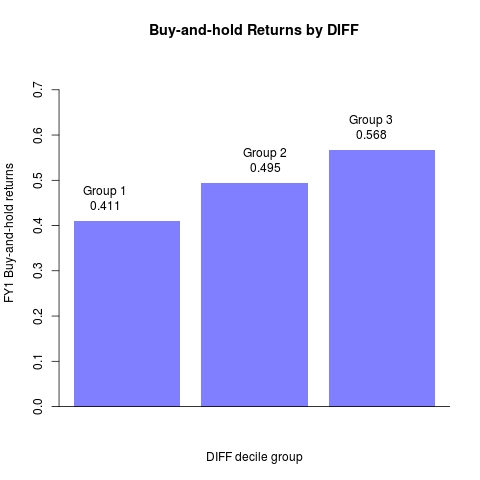
\includegraphics[height=2in, width=3in]{bahr-diff-decile2.jpeg}
\end{figure}
\end{center}
\end{frame}


\begin{frame}
\frametitle{Summary of Results}
\begin{enumerate}
\item Analyst forecasts are more accurate at shorter horizons, but statistical forecasts outperform at longer horizons
\item Analyst forecasts underperform statistical forecasts in the period prior to Reg-FD, consistent with a less favorable information environment
\item No clear relation between \emph{ex ante} uncertainty and relative forecast performance
\item Analyst forecasts perform better in high-tech, manufacturing, and healthcare
\item Statistical forecasts associated with marginally better contemporaneous returns
\end{enumerate}
\end{frame}

\begin{frame}
\frametitle{Conclusions and Extensions}
Analyst forecasts of earnings suffers from three flaws: 
\begin{enumerate}
\item Relatively simple to implement statistical models can beat analyst forecasts in terms of accuracy 
\item It is possible and useful to incorporate a wider information set than previous earnings into such models
\item Statistical models may give market participants who use them an advantage over those who rely on analyst forecasts
\end{enumerate}
Further Questions
\begin{itemize}
\item Unanswered: what do investors actually use to form expectations of firms' earnings?
\item Unanswered: do more accurate earnings forecasts from statistical models lead to better estimates of implied cost of capital or equity risk premia?
\end{itemize}
\end{frame}

\begin{frame}
\frametitle{Conclusions and Extensions}
Analyst forecasts of earnings suffers from three flaws: 
\begin{enumerate}
\item Relatively simple to implement statistical models can beat analyst forecasts in terms of accuracy 
\item It is possible and useful to incorporate a wider information set than previous earnings into such models
\item Statistical models may give market participants who use them an advantage over those who rely on analyst forecasts
\end{enumerate}
Further Questions
\begin{itemize}
\item Unanswered: what do investors actually use to form expectations of firms' earnings?
\item Unanswered: do more accurate earnings forecasts from statistical models lead to better estimates of implied cost of capital or equity risk premia?
\end{itemize}
\end{frame}

\begin{frame}
\frametitle{}
\begin{center}Thank you!\end{center}
\end{frame}

\begin{frame}
\frametitle{Summary Statistics}
\begin{table}
\Fontvi
\centering
\begin{tabular}{rrrrrr}
  \hline
 & mean & med & min & max & stdev \\ 
  \hline
EPS & 1.671 & 1.270 & -13.940 & 89.610 & 2.429 \\ 
  EPS Growth & 0.148 & 0.131 & -246.500 & 549 & 6.659 \\ 
  Total Assets & 11189.937 & 2859.255 & 0.808 & 797769 & 36046.376 \\ 
  Accruals & -0.034 & -0.037 & -5.224 & 1.864 & 0.115 \\ 
  Dividends & 4.294 & 0.333 & 0 & 18000 & 257.570 \\ 
  Dividend Payer & 0.241 & 0 & 0 & 1 & 0.428 \\ 
  Negative Earnings & 0.042 & 0 & 0 & 1 & 0.201 \\ 
  Delta Price & 0.095 & 0.050 & -2.033 & 9.529 & 0.510 \\ 
  return & 0.004 & 0.049 & -3.501 & 2.354 & 0.428 \\ 
  PE Ratio & 75.219 & 25 & -57200 & 151250 & 1896.962 \\ 
  GDP & 0.047 & 0.048 & -0.032 & 0.124 & 0.024 \\ 
  ROE & 0.739 & 0.159 & -312.626 & 5822.013 & 58.999 \\ 
  Unemployment & 0.062 & 0.056 & 0.038 & 0.108 & 0.018 \\ 
  Inflation (PPI) & 0.003 & 0.003 & -0.053 & 0.030 & 0.011 \\ 
  ales & 9900.868 & 2735.200 & -7.237 & 470171 & 27674.290 \\ 
  AR & 1900.042 & 363.594 & 0 & 418777 & 12828.263 \\ 
  AP & 980.353 & 182.422 & 0 & 149813 & 4173.909 \\ 
  Age & 18.231 & 17 & 5 & 32 & 8.479 \\ 
  $\Delta Sales$ & 1023.698 & 203 & -172892 & 278188 & 7136.501 \\ 
  $\Delta AR$ & 169.321 & 24.626 & -40708 & 60942 & 1778.590 \\ 
 $\Delta AP$ & 98.385 & 12.103 & -83588 & 71555 & 1376.945 \\ 
   \hline
\end{tabular}
\caption{Summary statistics of EPS and independent variables. $Age$ is number of years company is in the sample.}
\label{summary-stats}
\end{table}
\end{frame}


\begin{frame}
\frametitle{Methodology: Choosing Predictors}
\begin{table}
\Fontvi
\centering
\begin{tabular}{rrrrrr}
  \hline
 & mean & med & min & max & stdev \\ 
  \hline
$EPS_{t-1}$ & 0.8365 & 0.8903 & -0.1384 & 1.2728 & 0.2621 \\ 
  assets & 0.0316 & 0.0225 & -0.8275 & 0.3838 & 0.0877 \\ 
  Accruals & 1.0163 & 0.1647 & -27.7192 & 50.3953 & 5.7010 \\ 
  Dividends & -3.3222 & 0.0219 & -868.1679 & 21.1498 & 56.1218 \\ 
  Negative Earnings & 0.5258 & 0.2546 & -4.6542 & 7.1198 & 1.4530 \\ 
  $\Delta Price$ & 0.4812 & 0.2580 & -1.1649 & 5.5304 & 0.7044 \\ 
  return & 0.5376 & 0.2766 & -1.1905 & 9.9263 & 0.8845 \\ 
  PE Ratio & -0.0044 & -06 & -0.2647 & 0.0760 & 0.0213 \\ 
  GDP & 3.9724 & 1.8984 & -37.5517 & 144.6891 & 13.6927 \\ 
  ROE & 1.9134 & 0.8492 & -7.8009 & 18.1838 & 3.3770 \\ 
  Unemployment & -1.0157 & 0.1596 & -192.9481 & 678 & 21.0969 \\ 
  Inflation (PPI) & 10.4296 & 4.8584 & -108.8861 & 157.9932 & 22.9823 \\ 
  sales & 0.6885 & 0.4160 & -2.7407 & 7.1705 & 1.0305 \\ 
  AR & 0.0598 & 0.0324 & -0.7462 & 0.6187 & 0.1225 \\ 
  AP & 0.0656 & 0.0444 & -0.9054 & 0.6850 & 0.1384 \\ 
  $\Delta Sales$ & 04 & 01 & -0.0018 & 0.0066 & 08 \\ 
  $\Delta AR$ & 0.0014 & 04 & -0.0107 & 0.0359 & 0.0041 \\ 
$\Delta AP$ & 0.0020 & 06 & -0.0202 & 0.0523 & 0.0069 \\ 
   \hline
\end{tabular}
\caption{Estimated coefficients from regressions of the form $EPS_{t} = \alpha_0 + \alpha_{1}EPS_{t-1} + \alpha_{2}X_{t-1} +\varepsilon$.} 
\label{univariate-stats-eps}
\end{table}
\end{frame}


\end{document}
